\chapter{Algorytmy przetwarzania chmur punktów w systemach GIS}

\section{Pozyskiwanie danych}
Do pozyskiwania danych wykorzystuje się technologię LIDAR. Jest to nowoczesna metoda pozyskiwania informacji dotyczących wysokości terenu \cite{Marmol2003}. Efektem jej działania jest tzw “chmura punktów”, która uwzględnia wysokość nie tylko powierzchni ziemi, ale również drzew, budynków itp.

Dane zbierane są za pomocą aparatury umieszczonej w samolotach, na którą składają się odbiornik GPS służący do określania pozycji, czujnik INS pozwalający na określenie aktualnego przechyłu pojazdu oraz laser LRF mierzący odległość \cite{WBPW2012}. Laser emituje wiązkę w kierunku ziemi. Na podstawie czasu jaki minął między emisją wiązki a jej odczytem, określana jest odległość między aparaturą a badanym punktem. Jednocześnie zapisywane jest położenie skanera, co pozwala umieścić punkt w układzie odniesienia (np: WGS 84).

Urządzenia LIDAR pozwalają na rejestrację niemal dowolnych ilości tzw. impulsów pośrednich, które pochodzą np: od drzew. Dzięki temu chmura punktów pochodząca z jednego przelotu może posłużyć zarówno do utworzenia numerycznego modelu pokrycia terenu, jak również do utworzenia numerycznego modelu rzeźby terenu.

\begin{figure}[h!]
\centering
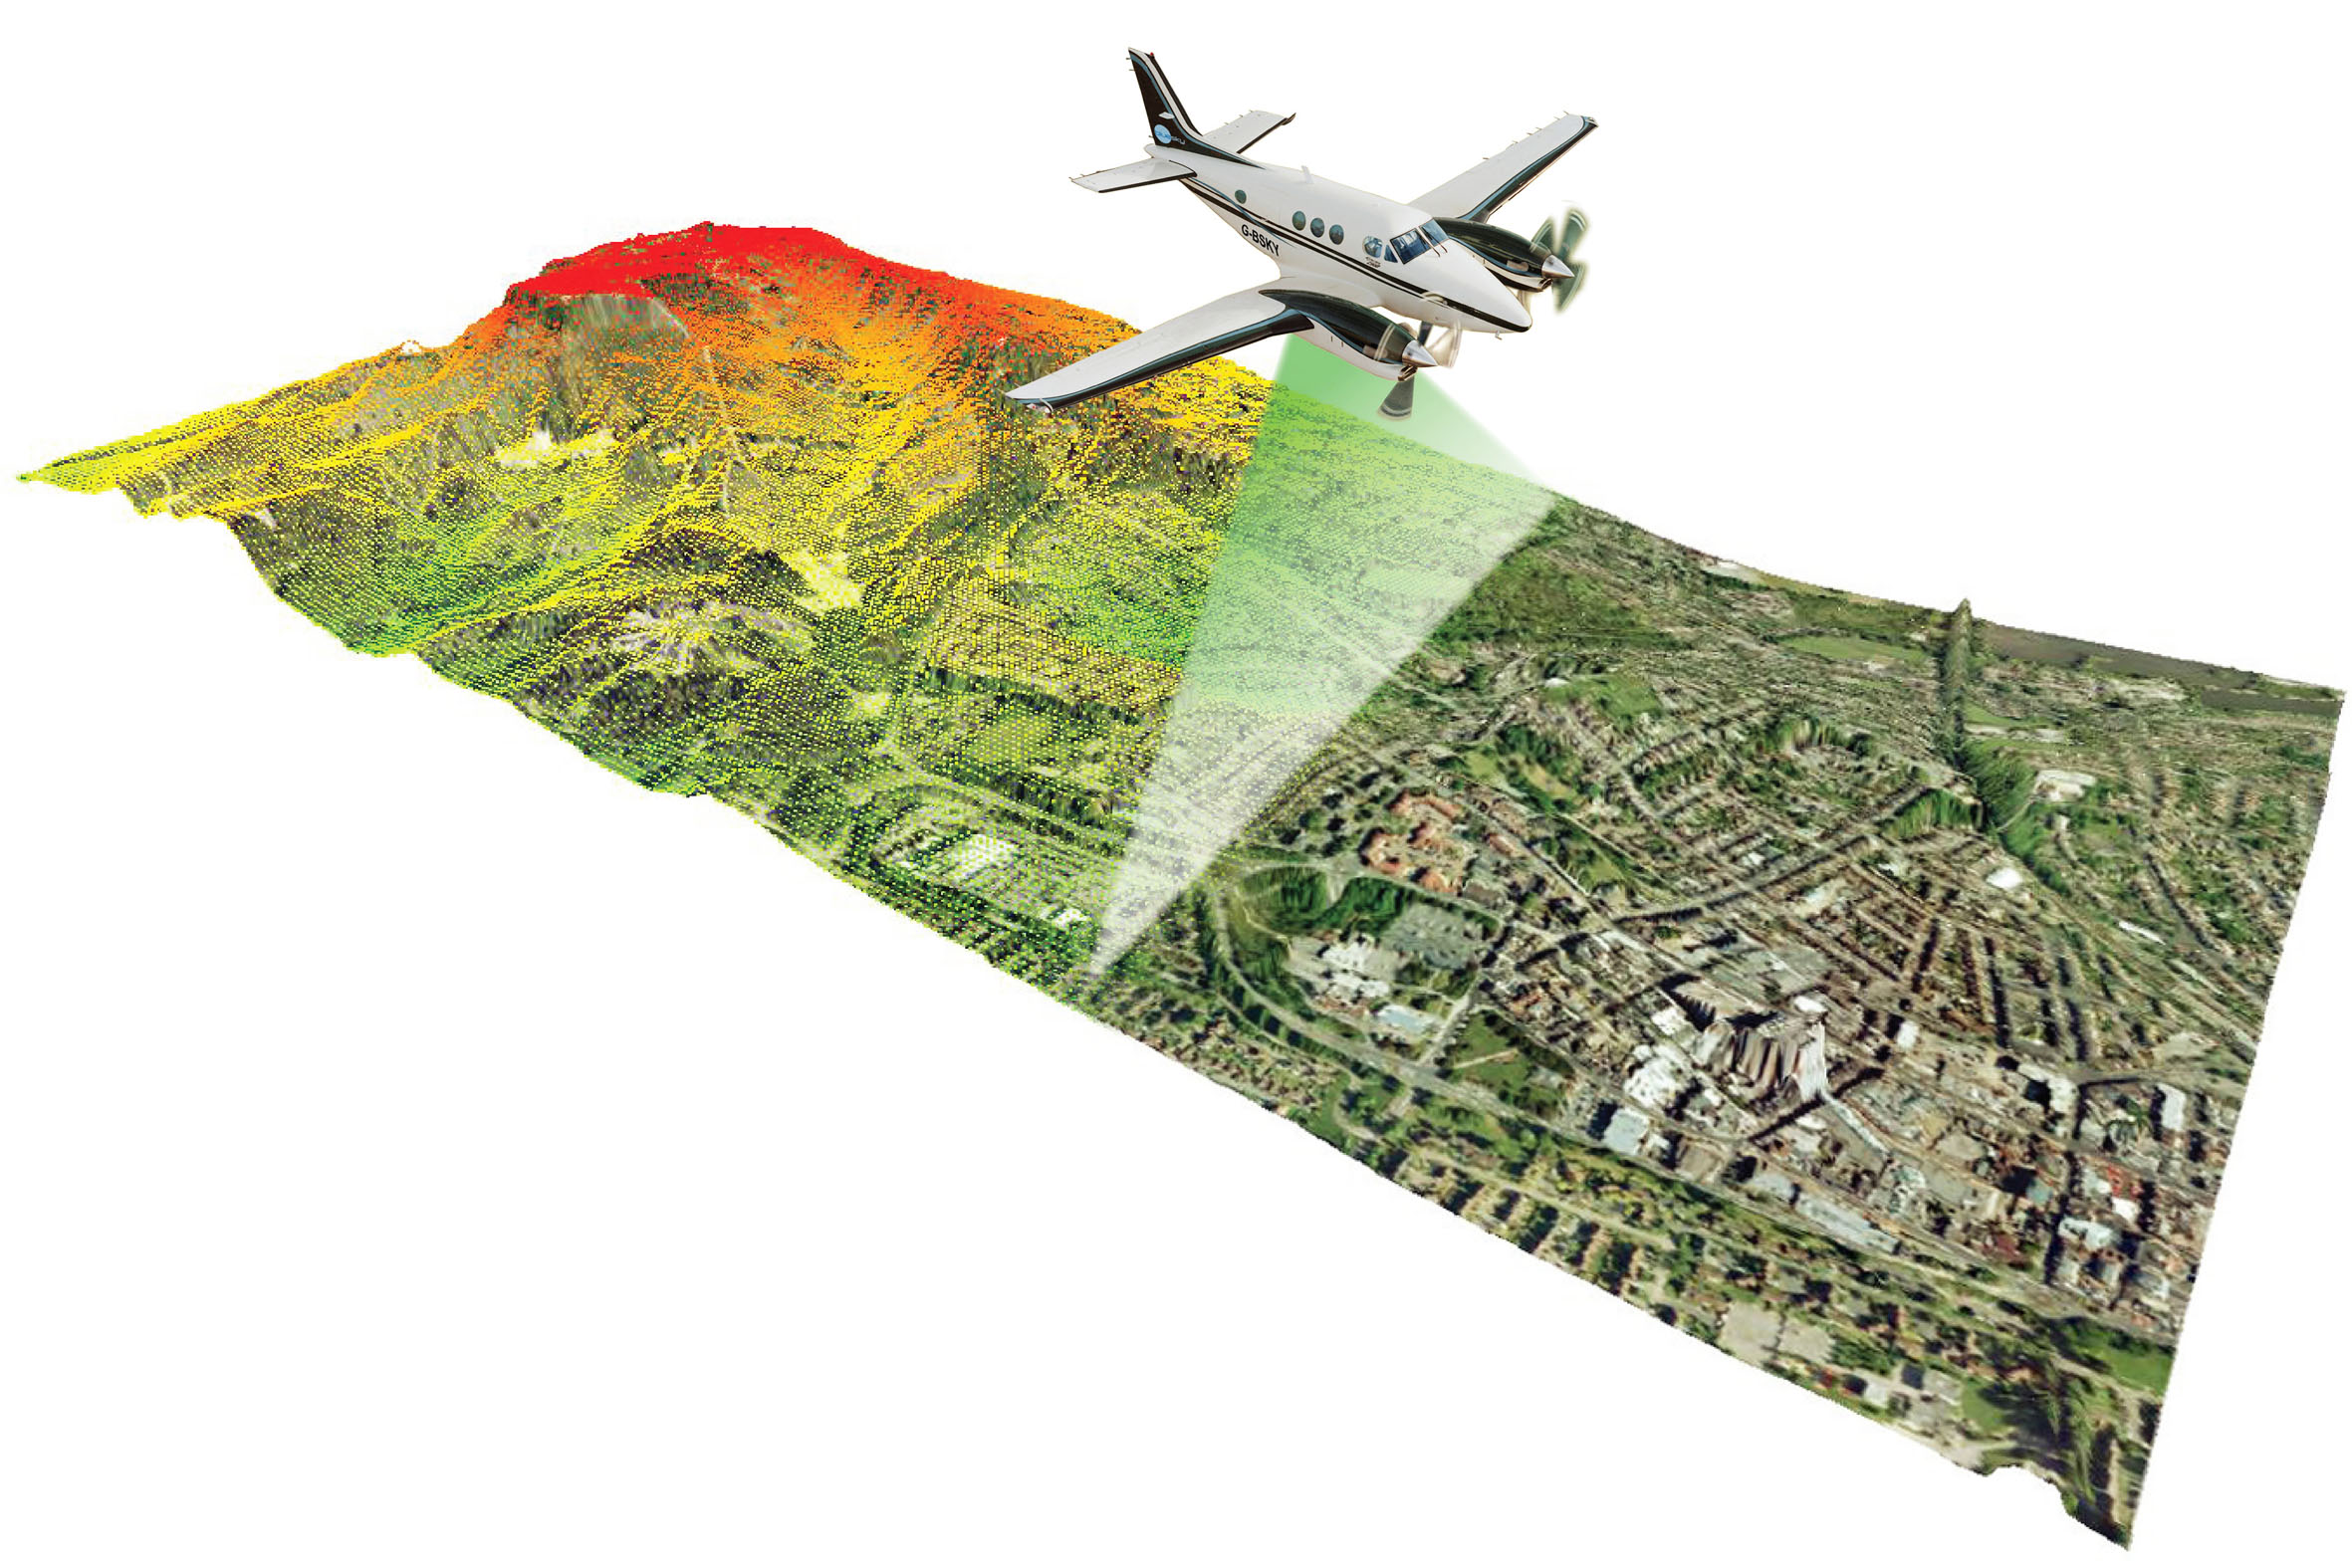
\includegraphics[width=1\textwidth]{img/LIDAR.jpg}
\caption{Schematycznie przedstawiony nalot podczas zbierania danych LIDAR}
\label{fig:lidar}
\end{figure}

Na rysunku \ref{fig:lidar} przedstawiono w sposób schematyczny jak przebiega pobieranie danych. Samolot podczas nalotu pobiera dane wzdłuż pewnego odcinka prostopadłego do kierunku lotu, z których następnie powstaje chmura punktów, której wizualizację również przedstawiono na rysunku.

\section{Opis wybranych algorytmów}

W poniższym rozdziale zostaną opisane istniejące algorytmy przetwarzania danych w postaci chmury punktów w systemach GIS.

\subsection{Triangulacja Delaunay'a}

Triangulacja Delaunay'a jest reprezentacją chmury punktów w postaci nieregularnej siatki trójkątów TIN (z ang. Triangulated Irregular Network). Jej cechą szczególną jest fakt, iż każdy z punktów znajduje się w wierzchołku przynajmniej jednego trójkąta \cite{Lee1980}. Triangulacja Delaunay'a jest często wykorzystywana przy przetwarzaniu danych LIDAR. Dzięki stosowaniu filtracji może służyć do oddzielania poszczególnych zbiorów punktów od siebie \cite{koziol2007} bądź też do znajdywania łamanej otaczającej zadany zbiór punktów \cite{website:HumanGeoBlog}. Istnieje wiele implementacji algorytmu pozwalającego na przetworzenie chmury punktów do postaci siatki trójkątów \cite{Lee1980,Dwyer1987,jiang2010}. W artykule \cite{Lee1980} opisano dwa algorytmy tworzenia takiej siatki - dziel i zwyciężaj oraz tribuild. Pierwszy z nich o złożoności obliczeniowej $O(N log N)$ rekurencyjnie dzieli zbiór punktów pośrednich na mniejsze zbiory, w nich dokonuje triangulacji a następnie łączy je. Drugi z nich o złożoności obliczeniowej $O(N^{3/2})$ zakłada znajomość prostokąta który otacza zadany zbiór punktów. Prostokąt ten jest dzielony na mniejsze, a następnie dla każdego mniejszego prostokąta:

\begin{algorithmic}
    \For {punkt P w punktach należących do prostokąta}
    \If {P jedyny punkt w prostokącie}
        \State połącz punkt z wierzchołkami prostokąta
    \Else
        \State dodaj krawędzie, aby nie zniszczyć triangulacji
    \EndIf
    \EndFor
\end{algorithmic}

Przykładowe kolejne etapy tak przeprowadzonej triangulacji pokazano na rysunku \ref{fig:iter_triangulacja}.

\begin{figure}[h!]
    \centering
    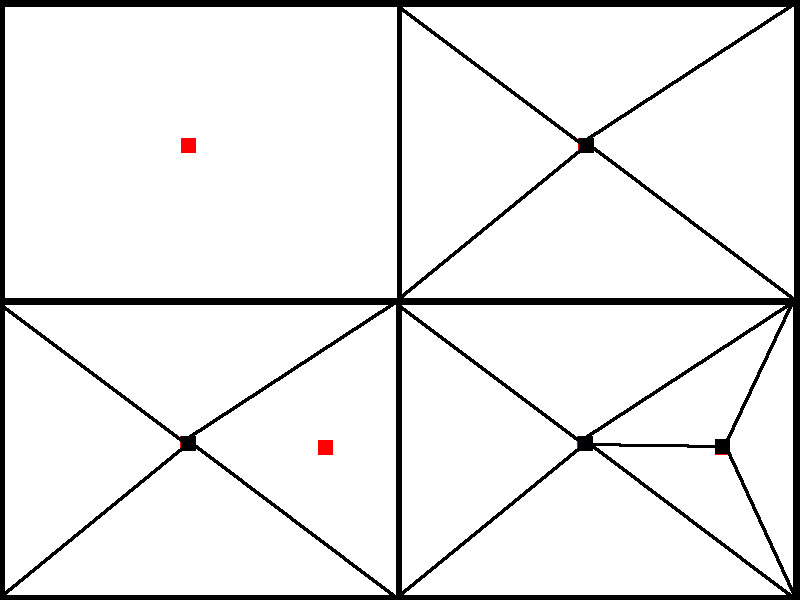
\includegraphics[width=0.5\textwidth]{img/iter_triangulacja.jpg}
    \caption{Iteracyjna triangulacja}
    \label{fig:iter_triangulacja}
\end{figure}



\subsection{Metoda2}

\subsection{Metoda3}

\section{Klasyfikacja danych}
